\chapter{Description of BER Test Setup}
\label{sec:appendxi_setup}
The major components from the block diagram shown in Figure \ref{fig:LabTestBlock} functions are summarized as follows:
\begin{itemize}
\item The \textbf{SOQPSK-TG Transmitter} is a PAQ enabled L-band transmitter shown in Figure \ref{fig:trans}.
\item The \textbf{Multipath Channel} emulator generates multipath interference for a given channel at RF shown in Figure \ref{fig:emu}.
\item The \textbf{Noise Source} generates calibrated additive white Gaussian noise for a given $\text{E}_\text{b}/\text{N}_\text{0}$ shown in Figure \ref{fig:noise}.
\item The \textbf{Power Splitter} split the power between the Spectrum Analyzer and the T/M Receiver \& Demodulator  shown in Figure \ref{fig:splitter}.
\item The \textbf{Spectrum Analyzer} showed the power spectrum of the multipath channel shown in Figure \ref{fig:specAn}.
\item The \textbf{T/M Receiver \& Demodulator} produced the no equalization bits at $10.3125$ Mbits/s and down-converted RF to $70$ MHz IF  shown in Figure \ref{fig:HostSystem}.
\item The \textbf{Preamble Scrubber} explained in \cite{hog2016} locates and removes the preamble and ASM in the $10.3125$ Mbits/s to produce a data bit stream at $10$ Mbits/s shown in Figure \ref{fig:scrubber}.
\item The \textbf{BERT} computes the BER for six bit streams shown in Figure \ref{fig:BERT}.
\end{itemize}
\clearpage
\begin{figure}
	\centering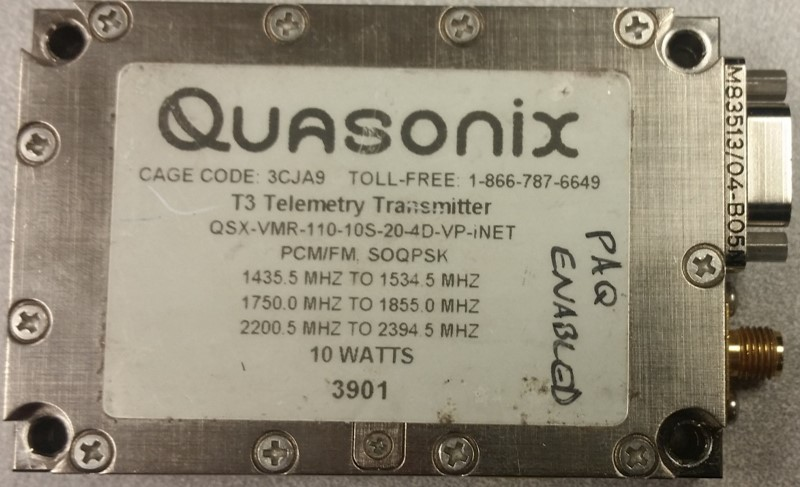
\includegraphics[scale=0.5]{figures/eq_GPUimplementation/trans.jpg}
	\caption{The SOQPSK-TG transmitter is a PAQ enabled L-band transmitter. The transmitted bits has the PAQ packet structure with a repeated pn11 data sequence repeated almost three times per packet. The transmitter was connected directly into the channel emulator. The transmitter was manufactured by Quasonix: QSX VMR 110 00S 20 2D VP iNET S/N 3901.}
	\label{fig:trans}
\end{figure}
\begin{figure}
	\centering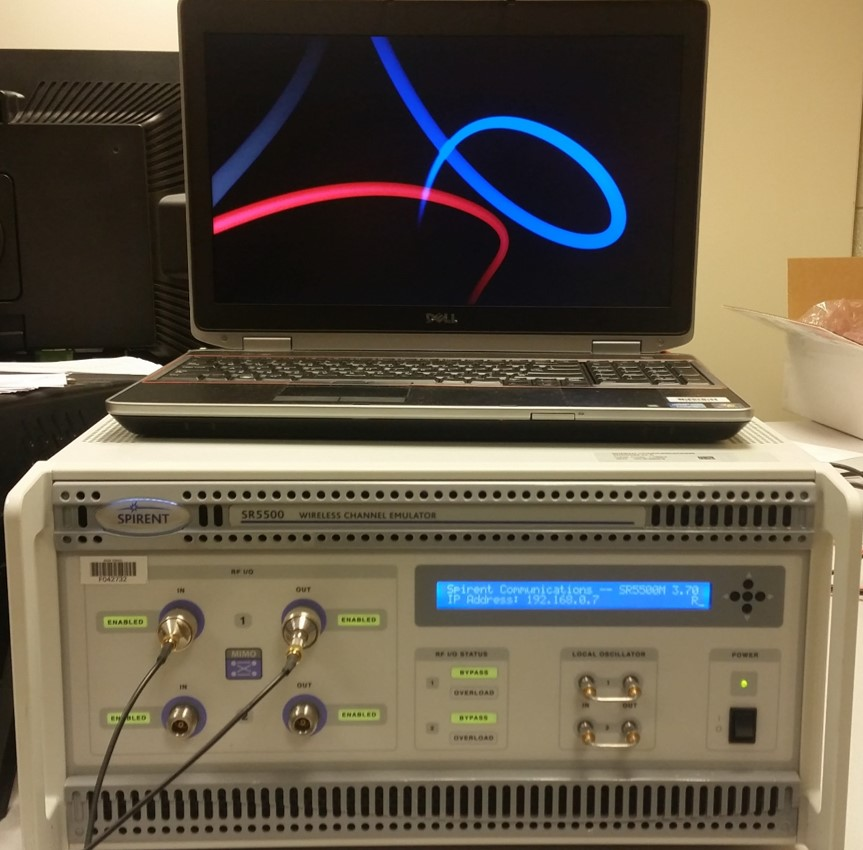
\includegraphics[scale=0.5]{figures/eq_GPUimplementation/emu.jpg}
	\caption{The multipath channel emulator generates multipath interference for a given channel at RF. The given channel parameters for these static tests were attenuation, delay, and phase. All other parameters were left default. The channel emulator was connected directly to the noise source. The channel emulator was manufactured by Spirint: SR 5500.}
	\label{fig:emu}
\end{figure}
\begin{figure}
	\centering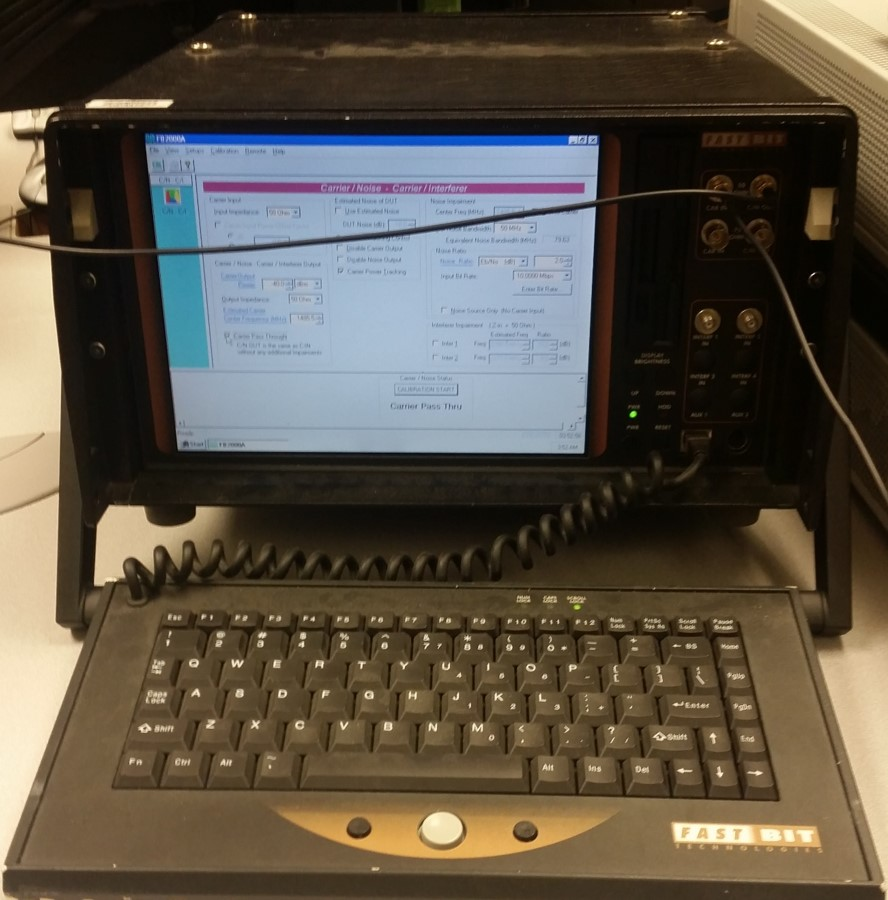
\includegraphics[scale=0.5]{figures/eq_GPUimplementation/noise.jpg}
	\caption{The noise source generates calibrated additive white Gaussian noise for a given $\text{E}_\text{b}/\text{N}_\text{0}$. The only parameters required for the noise source was the bit rate ($10.3125$Mbps) and $\text{E}_\text{b}/\text{N}_\text{0}$ in dB. The noise source was connected to the power splitter. The calibrated noise source was manufactured by Fast Bit: FB0008.}
	\label{fig:noise}
\end{figure}
\begin{figure}
	\centering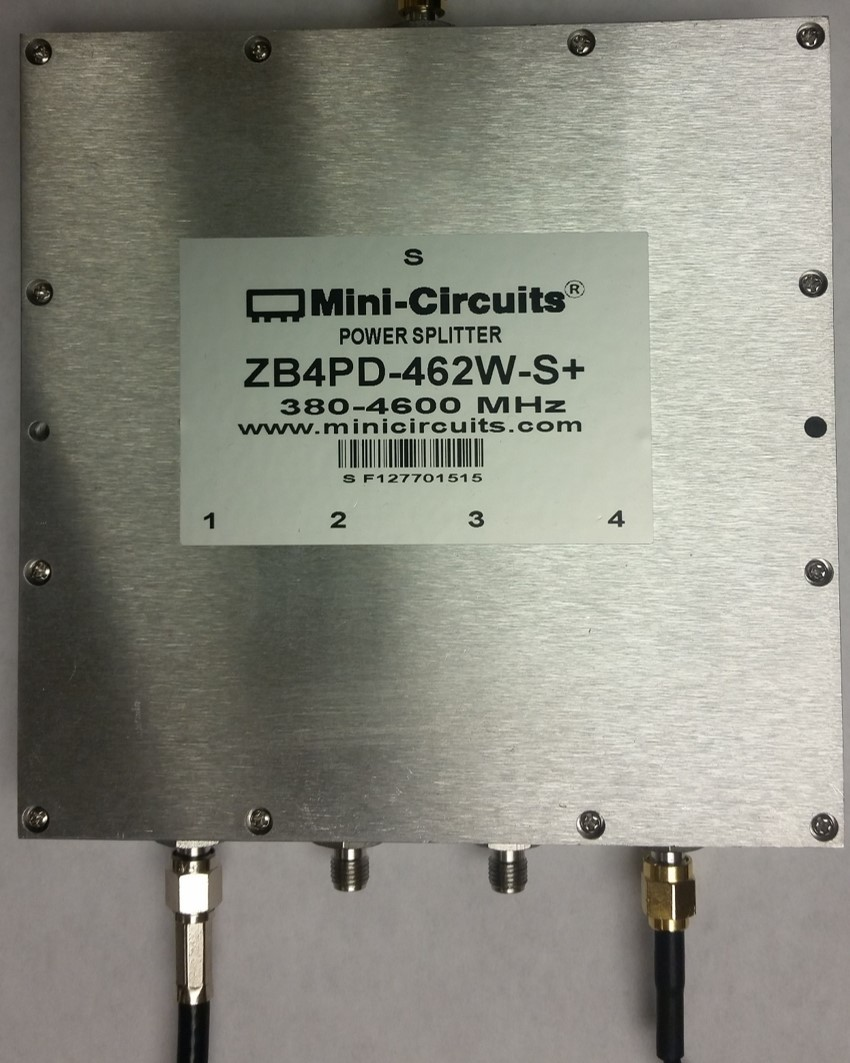
\includegraphics[scale=0.5]{figures/eq_GPUimplementation/splitter.jpg}
	\caption{The power splitter split the power between the Spectrum Analyzer and the T/M Receiver \& Demodulator. The power splitter was manufactured by Mini-circuits: ZB4PD-462W-S+.}
	\label{fig:splitter}
\end{figure}
\begin{figure}
	\centering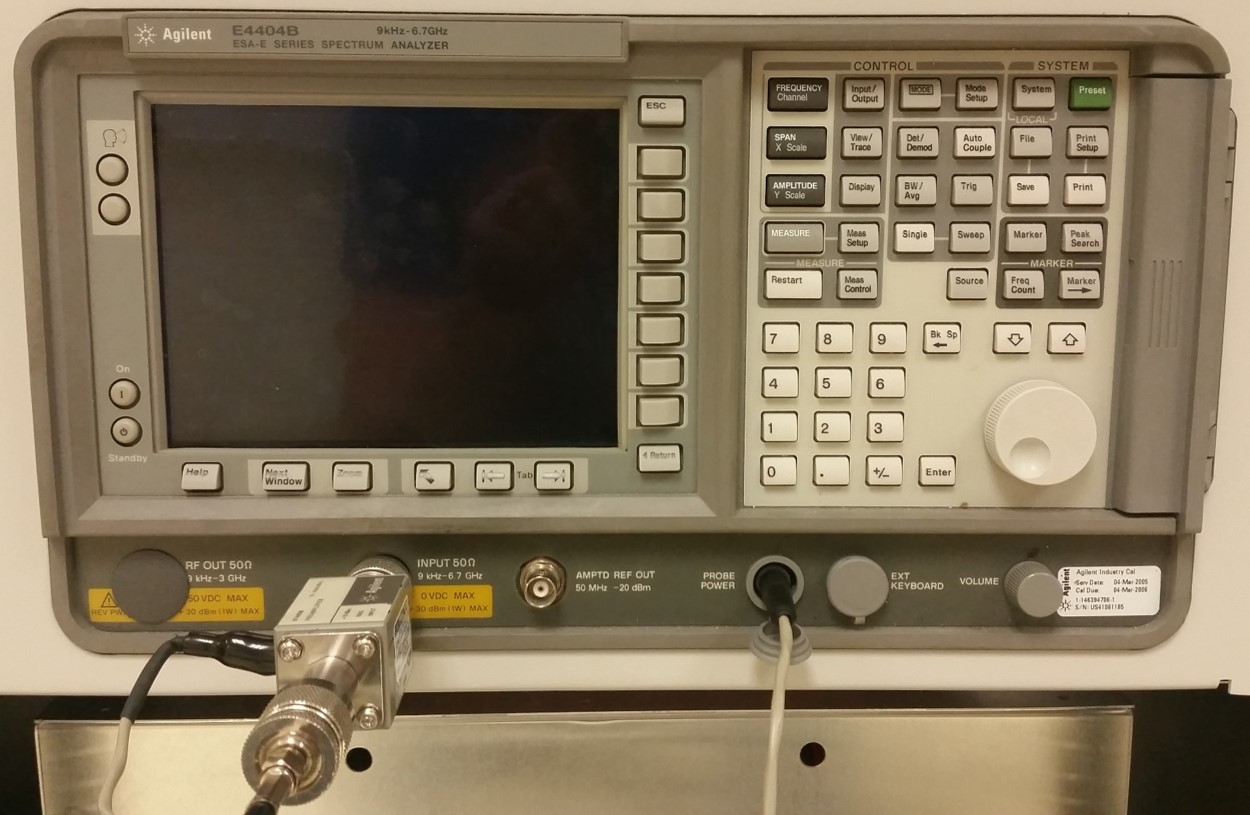
\includegraphics[scale=0.5]{figures/eq_GPUimplementation/specAn.jpg}
	\caption{The spectrum analyzer showed the power spectrum of the multipath channel manufactured by Agilent: E4404B ESA-E Series Spectrum Analyzer.}
	\label{fig:specAn}
\end{figure}
\begin{figure}
	\centering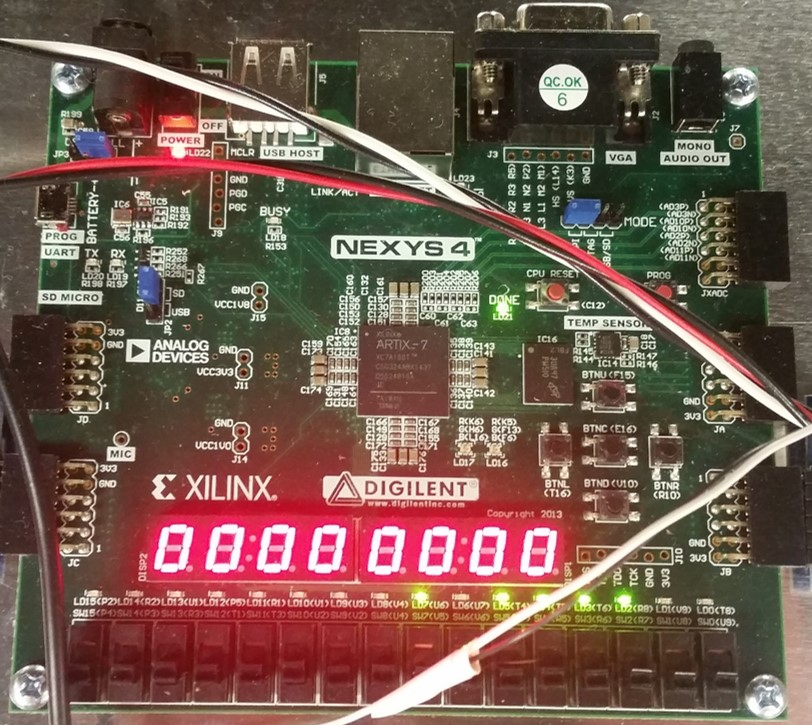
\includegraphics[scale=0.5]{figures/eq_GPUimplementation/scrubber.jpg}
	\caption{The preamble scrubber explained in \cite{hog2016} locates and removes the preamble and ASM in the $10.3125$ Mbits/s to produce a data bit stream at $10$ Mbits/s. The FPGA was manufactured by Xilinx}
	\label{fig:scrubber}
\end{figure}
\begin{figure}
	\centering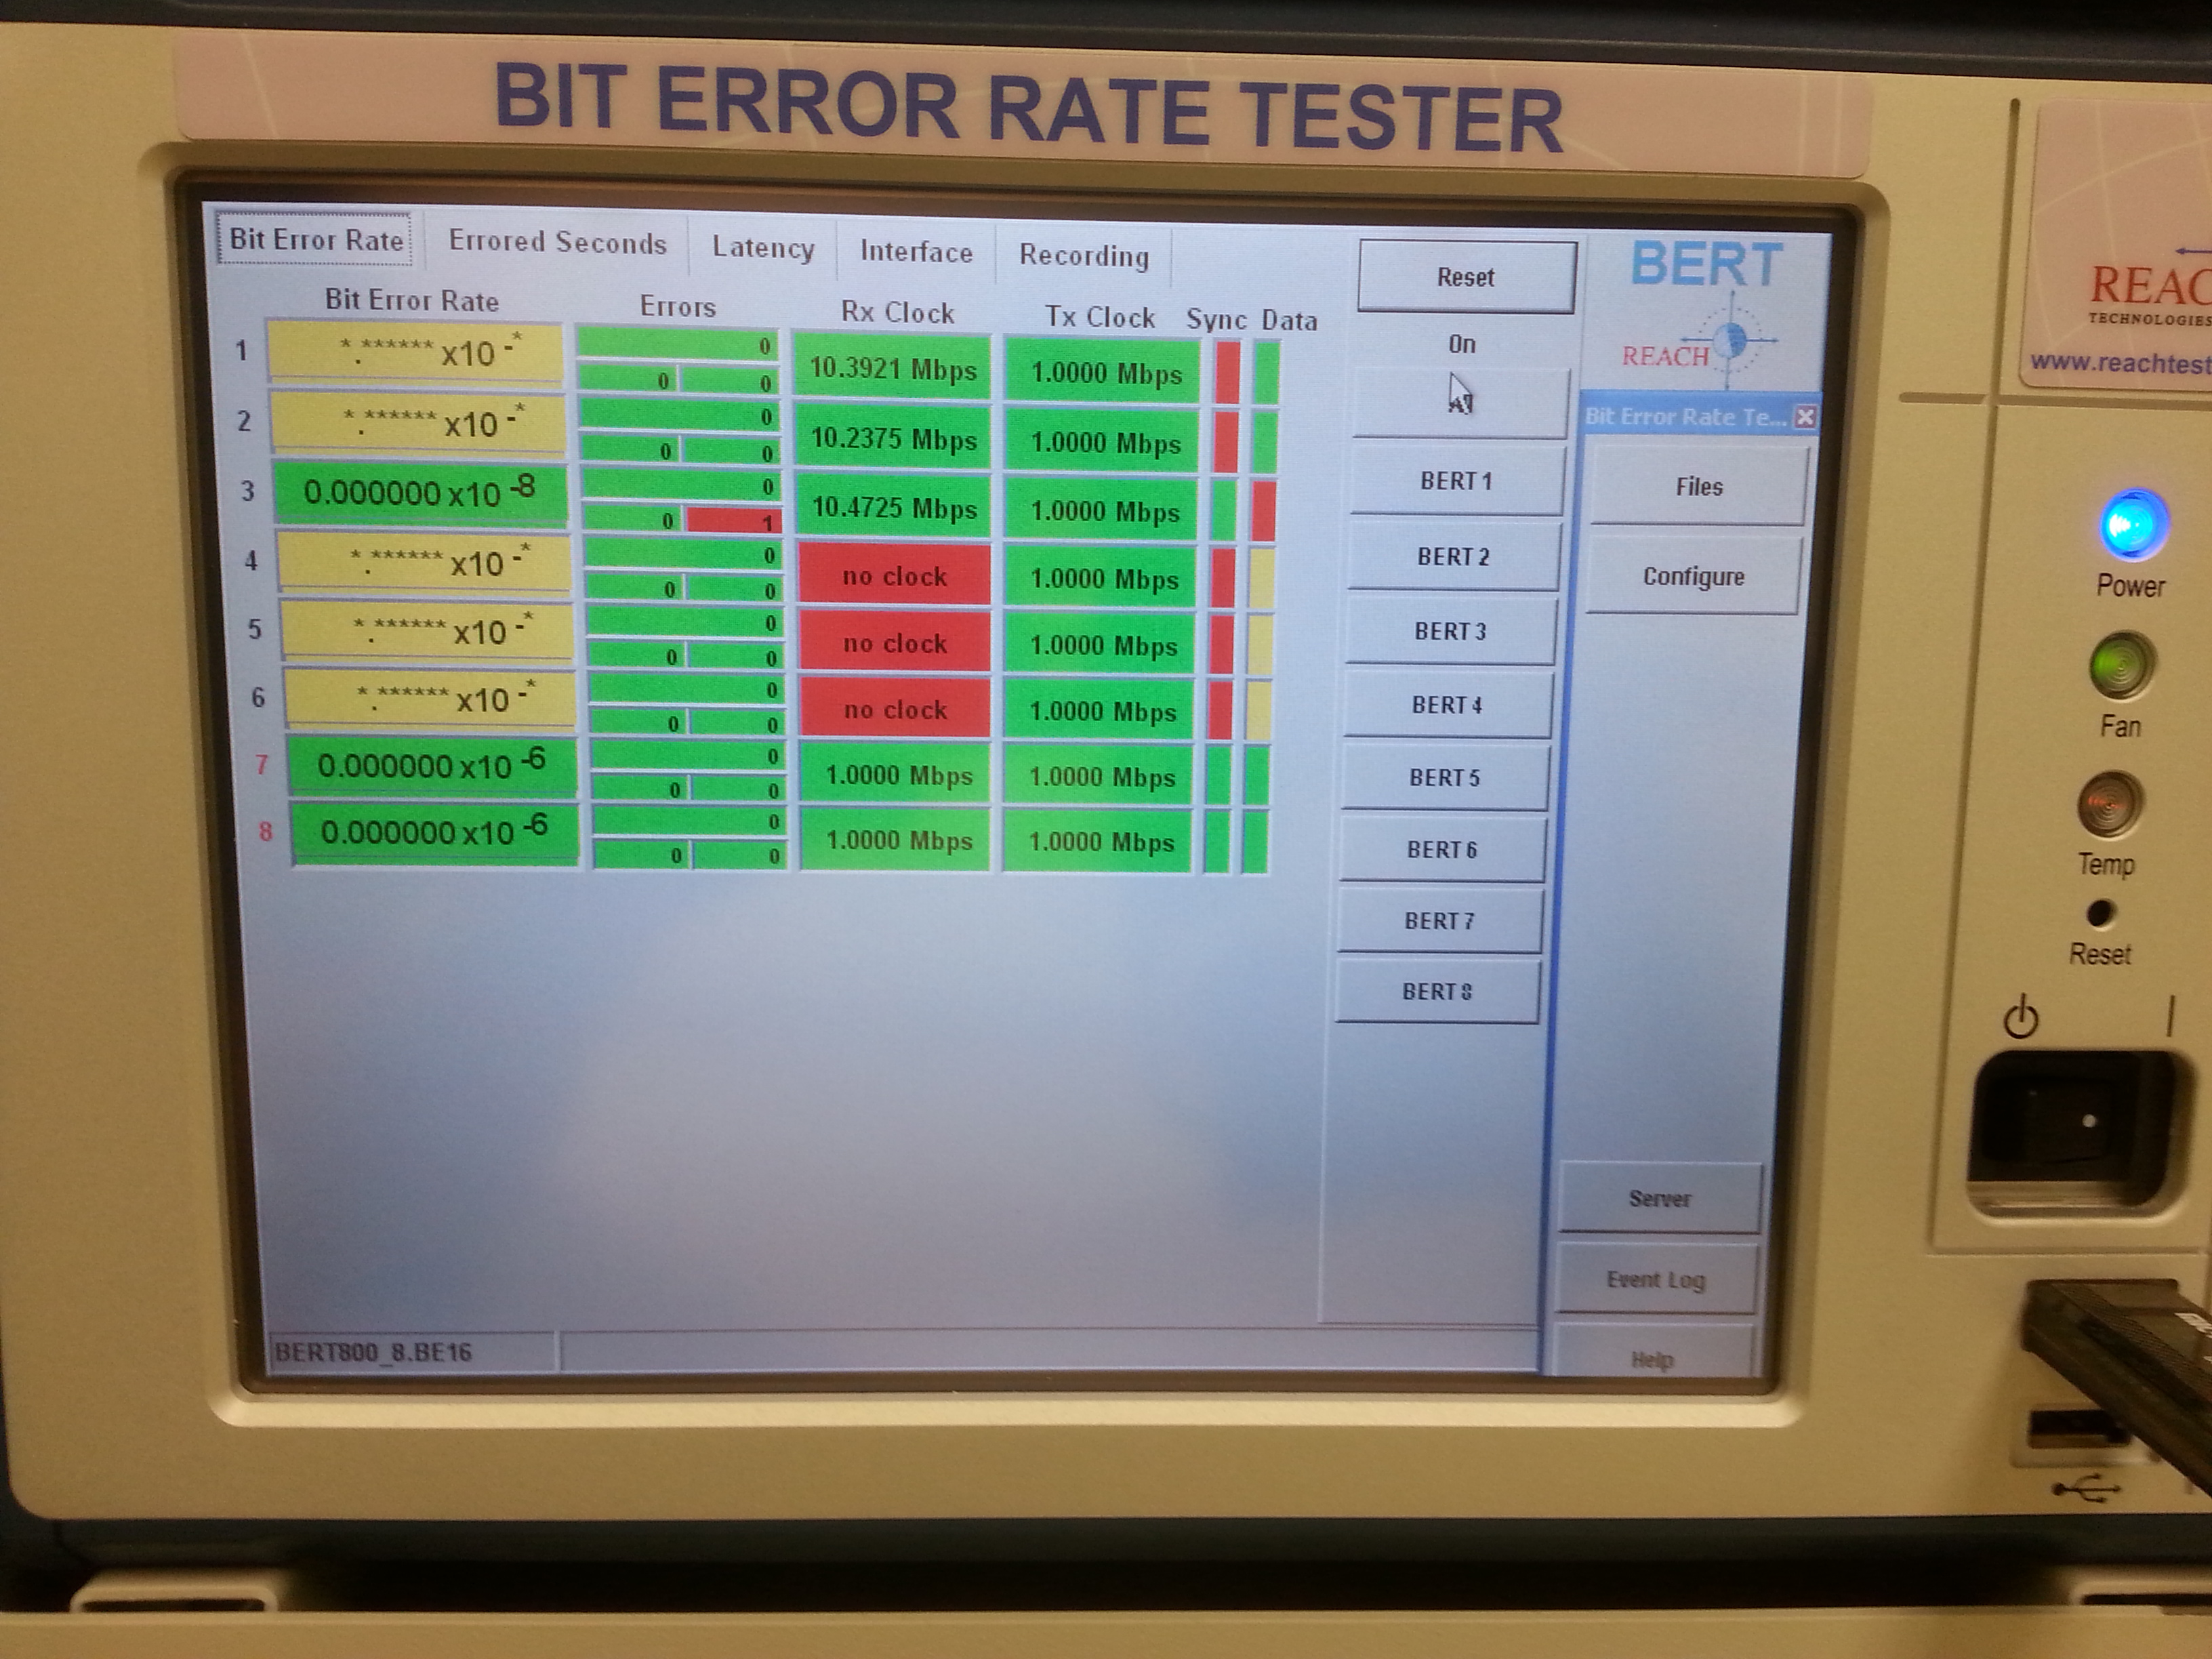
\includegraphics[scale=0.1]{figures/eq_GPUimplementation/20150912_194530.jpg}
	\caption{The BERT (bit error rate tester) computes the BER for six bit streams manufactured by Reach Technologies.}
	\label{fig:BERT}
\end{figure}

